
\begin{figure}[h]
    \centering
    \begin{subfigure}[t]{0.4\textwidth}
    \captionsetup{justification=centering}
        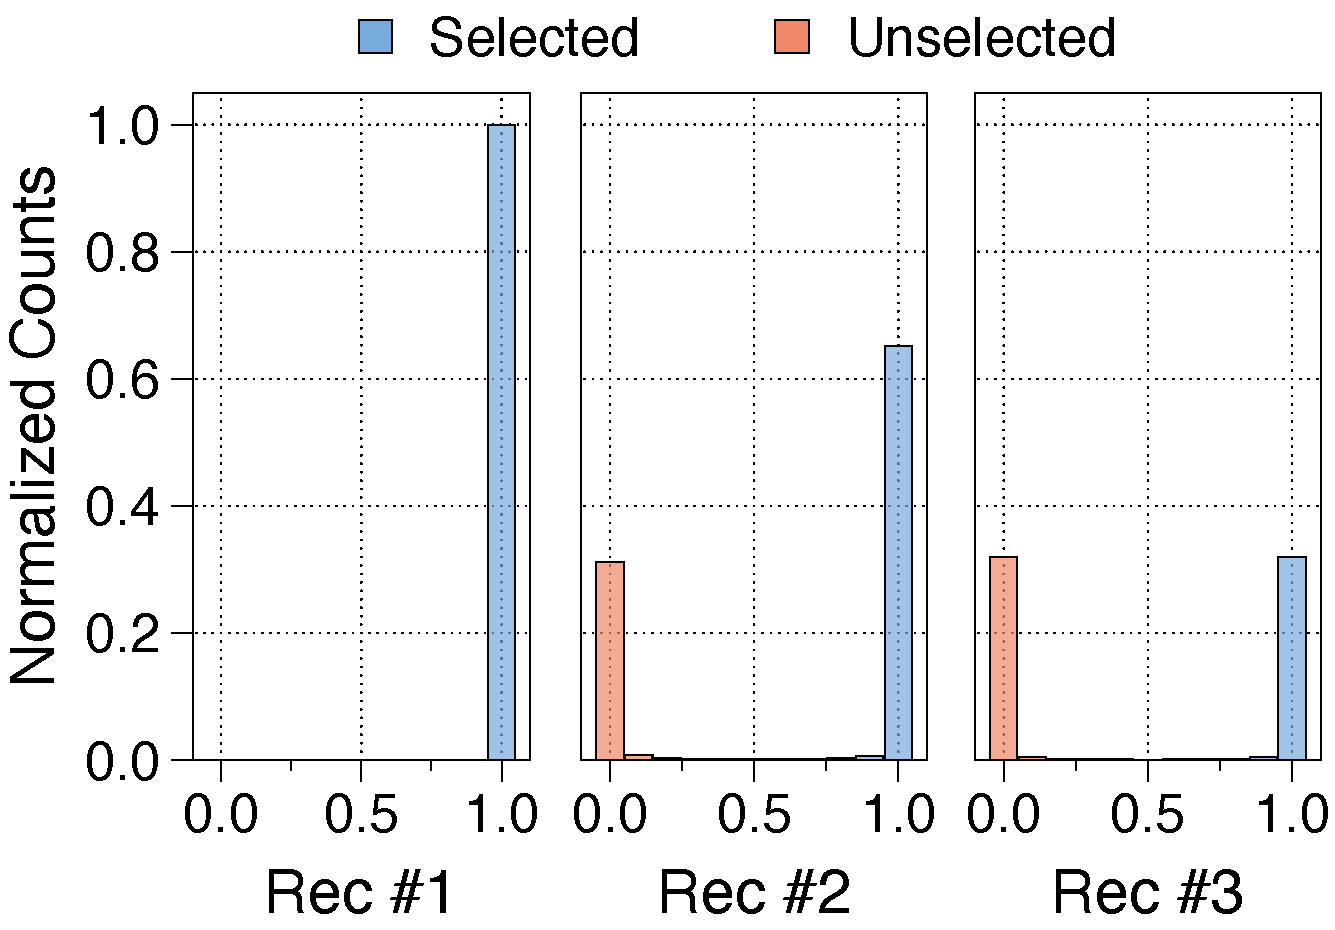
\includegraphics[width=\textwidth]{figs/weight_values/aux_loss_expert_app.pdf}
        \subcaption{Expert-choice (Auxiliary loss)}
    \end{subfigure}
    \centering
    \hspace{25pt}
    \begin{subfigure}[t]{0.4\textwidth}
    \captionsetup{justification=centering}
        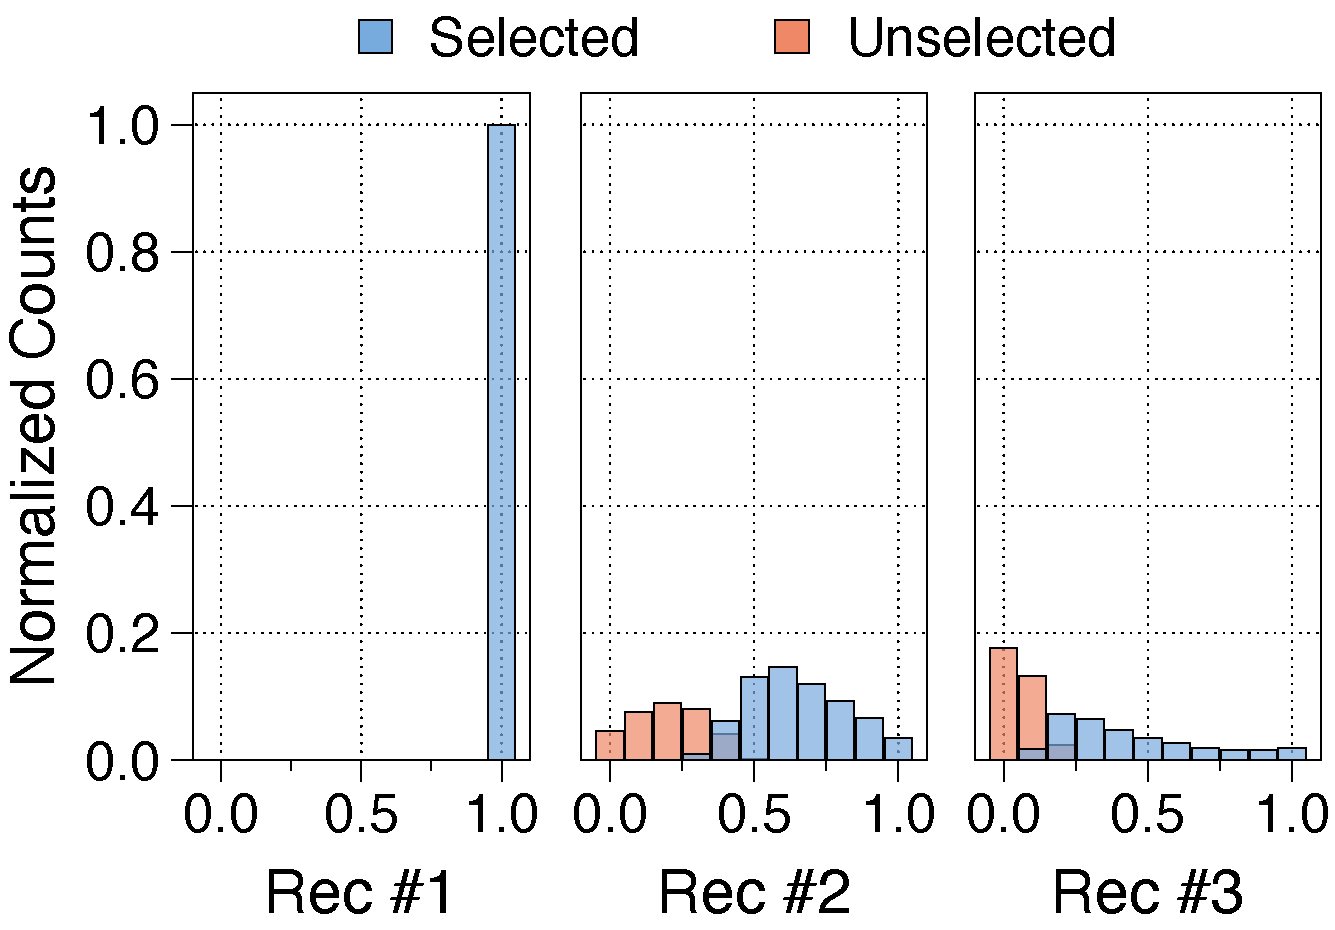
\includegraphics[width=\textwidth]{figs/weight_values/aux_router_expert_app.pdf}
        \subcaption{Expert-choice (Auxiliary router)}
    \end{subfigure}
    \centering
    \begin{subfigure}[t]{0.4\textwidth}
    \captionsetup{justification=centering}
        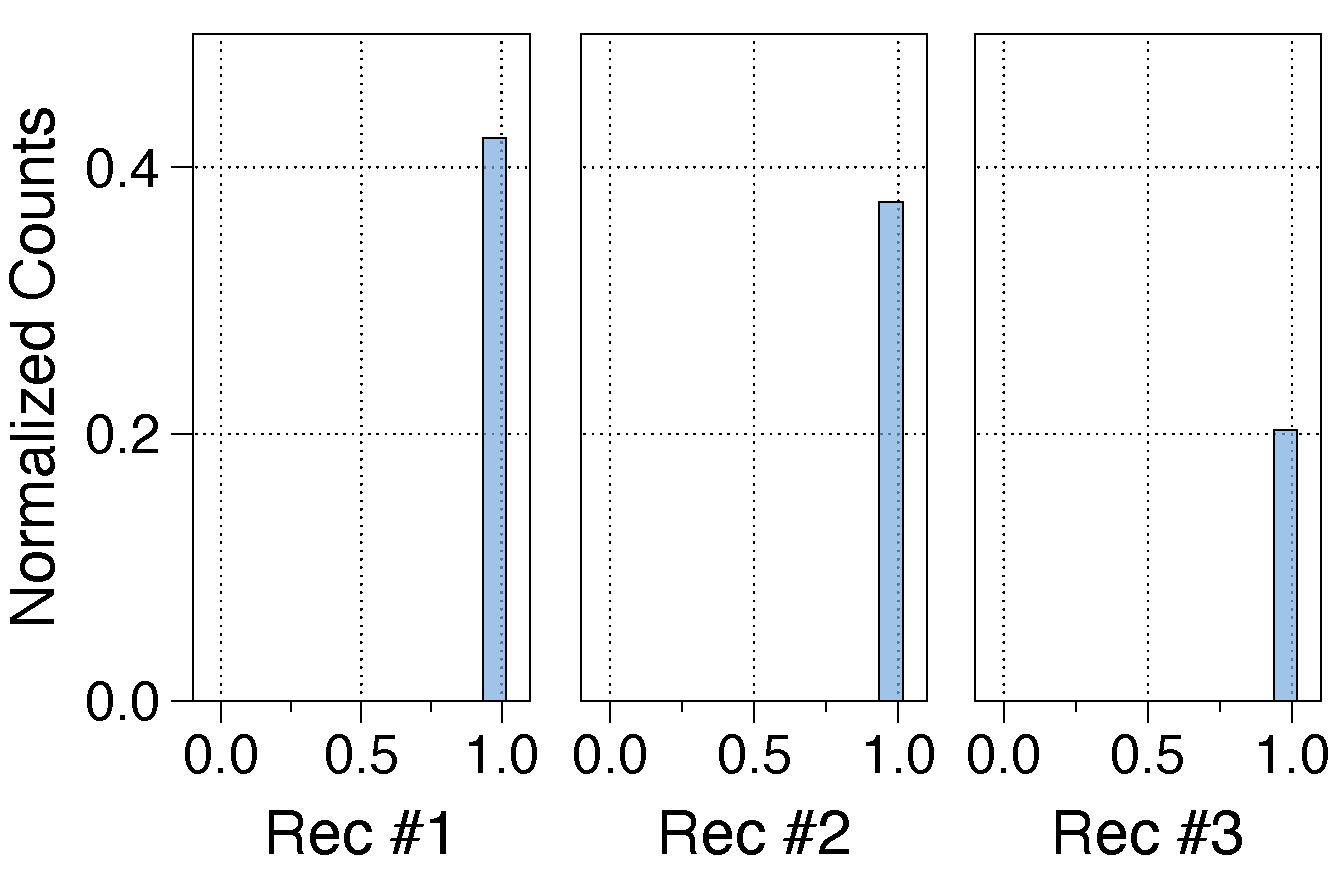
\includegraphics[width=\textwidth]{figs/weight_values/bal_loss_token_app.pdf}
        \subcaption{Token-choice (Balancing loss)}
    \end{subfigure}
    \centering
    \hspace{25pt}
    \begin{subfigure}[t]{0.4\textwidth}
    \captionsetup{justification=centering}
        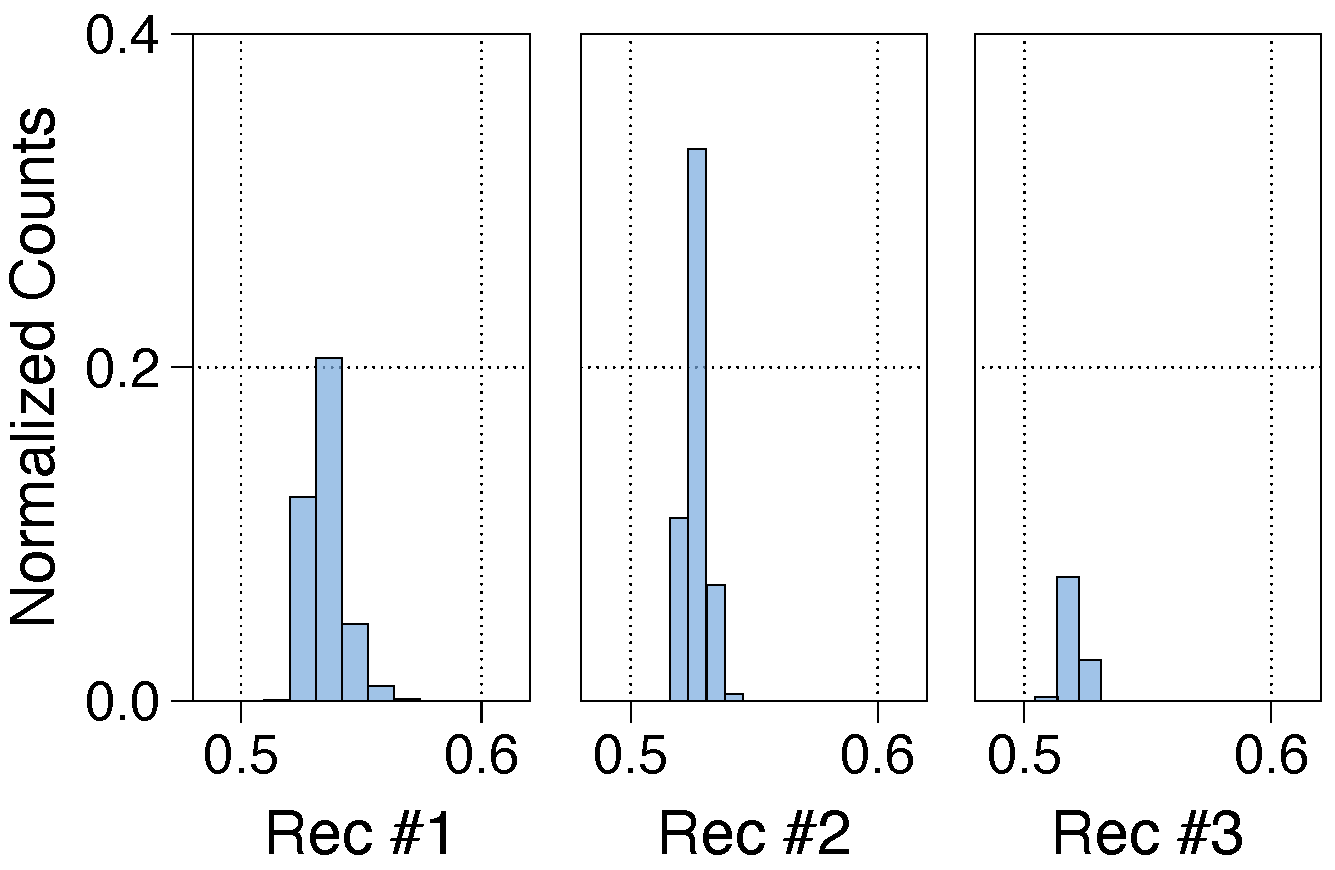
\includegraphics[width=\textwidth]{figs/weight_values/loss_free_token_app.pdf}
        \subcaption{Token-choice (Loss-free)}
    \end{subfigure}
    \caption{
    Distribution of router weights for selected and unselected tokens at each recursion step in expert-choice and token-choice MoR~($N_r$=3). All models use the recursion-wise KV caching strategy. The subplots show results for (a) expert-choice routing with auxiliary loss, (b) auxiliary router, (c) token-choice routing with balancing loss, and (d) loss-free algorithm. Each subplot uses the best hyperparameter settings identified in \autoref{tab:ablation_study_router}.
    }    
    \label{fig:weight_values_app}
\end{figure}

